% Options for packages loaded elsewhere
\PassOptionsToPackage{unicode}{hyperref}
\PassOptionsToPackage{hyphens}{url}
%
\documentclass[
  10pt,
]{article}
\usepackage{amsmath,amssymb}
\usepackage{iftex}
\ifPDFTeX
  \usepackage[T1]{fontenc}
  \usepackage[utf8]{inputenc}
  \usepackage{textcomp} % provide euro and other symbols
\else % if luatex or xetex
  \usepackage{unicode-math} % this also loads fontspec
  \defaultfontfeatures{Scale=MatchLowercase}
  \defaultfontfeatures[\rmfamily]{Ligatures=TeX,Scale=1}
\fi
\usepackage{lmodern}
\ifPDFTeX\else
  % xetex/luatex font selection
\fi
% Use upquote if available, for straight quotes in verbatim environments
\IfFileExists{upquote.sty}{\usepackage{upquote}}{}
\IfFileExists{microtype.sty}{% use microtype if available
  \usepackage[]{microtype}
  \UseMicrotypeSet[protrusion]{basicmath} % disable protrusion for tt fonts
}{}
\makeatletter
\@ifundefined{KOMAClassName}{% if non-KOMA class
  \IfFileExists{parskip.sty}{%
    \usepackage{parskip}
  }{% else
    \setlength{\parindent}{0pt}
    \setlength{\parskip}{6pt plus 2pt minus 1pt}}
}{% if KOMA class
  \KOMAoptions{parskip=half}}
\makeatother
\usepackage{xcolor}
\usepackage[margin=0.65in]{geometry}
\usepackage{color}
\usepackage{fancyvrb}
\newcommand{\VerbBar}{|}
\newcommand{\VERB}{\Verb[commandchars=\\\{\}]}
\DefineVerbatimEnvironment{Highlighting}{Verbatim}{commandchars=\\\{\}}
% Add ',fontsize=\small' for more characters per line
\newenvironment{Shaded}{}{}
\newcommand{\AlertTok}[1]{\textcolor[rgb]{1.00,0.00,0.00}{\textbf{#1}}}
\newcommand{\AnnotationTok}[1]{\textcolor[rgb]{0.38,0.63,0.69}{\textbf{\textit{#1}}}}
\newcommand{\AttributeTok}[1]{\textcolor[rgb]{0.49,0.56,0.16}{#1}}
\newcommand{\BaseNTok}[1]{\textcolor[rgb]{0.25,0.63,0.44}{#1}}
\newcommand{\BuiltInTok}[1]{\textcolor[rgb]{0.00,0.50,0.00}{#1}}
\newcommand{\CharTok}[1]{\textcolor[rgb]{0.25,0.44,0.63}{#1}}
\newcommand{\CommentTok}[1]{\textcolor[rgb]{0.38,0.63,0.69}{\textit{#1}}}
\newcommand{\CommentVarTok}[1]{\textcolor[rgb]{0.38,0.63,0.69}{\textbf{\textit{#1}}}}
\newcommand{\ConstantTok}[1]{\textcolor[rgb]{0.53,0.00,0.00}{#1}}
\newcommand{\ControlFlowTok}[1]{\textcolor[rgb]{0.00,0.44,0.13}{\textbf{#1}}}
\newcommand{\DataTypeTok}[1]{\textcolor[rgb]{0.56,0.13,0.00}{#1}}
\newcommand{\DecValTok}[1]{\textcolor[rgb]{0.25,0.63,0.44}{#1}}
\newcommand{\DocumentationTok}[1]{\textcolor[rgb]{0.73,0.13,0.13}{\textit{#1}}}
\newcommand{\ErrorTok}[1]{\textcolor[rgb]{1.00,0.00,0.00}{\textbf{#1}}}
\newcommand{\ExtensionTok}[1]{#1}
\newcommand{\FloatTok}[1]{\textcolor[rgb]{0.25,0.63,0.44}{#1}}
\newcommand{\FunctionTok}[1]{\textcolor[rgb]{0.02,0.16,0.49}{#1}}
\newcommand{\ImportTok}[1]{\textcolor[rgb]{0.00,0.50,0.00}{\textbf{#1}}}
\newcommand{\InformationTok}[1]{\textcolor[rgb]{0.38,0.63,0.69}{\textbf{\textit{#1}}}}
\newcommand{\KeywordTok}[1]{\textcolor[rgb]{0.00,0.44,0.13}{\textbf{#1}}}
\newcommand{\NormalTok}[1]{#1}
\newcommand{\OperatorTok}[1]{\textcolor[rgb]{0.40,0.40,0.40}{#1}}
\newcommand{\OtherTok}[1]{\textcolor[rgb]{0.00,0.44,0.13}{#1}}
\newcommand{\PreprocessorTok}[1]{\textcolor[rgb]{0.74,0.48,0.00}{#1}}
\newcommand{\RegionMarkerTok}[1]{#1}
\newcommand{\SpecialCharTok}[1]{\textcolor[rgb]{0.25,0.44,0.63}{#1}}
\newcommand{\SpecialStringTok}[1]{\textcolor[rgb]{0.73,0.40,0.53}{#1}}
\newcommand{\StringTok}[1]{\textcolor[rgb]{0.25,0.44,0.63}{#1}}
\newcommand{\VariableTok}[1]{\textcolor[rgb]{0.10,0.09,0.49}{#1}}
\newcommand{\VerbatimStringTok}[1]{\textcolor[rgb]{0.25,0.44,0.63}{#1}}
\newcommand{\WarningTok}[1]{\textcolor[rgb]{0.38,0.63,0.69}{\textbf{\textit{#1}}}}
\usepackage{longtable,booktabs,array}
\usepackage{calc} % for calculating minipage widths
% Correct order of tables after \paragraph or \subparagraph
\usepackage{etoolbox}
\makeatletter
\patchcmd\longtable{\par}{\if@noskipsec\mbox{}\fi\par}{}{}
\makeatother
% Allow footnotes in longtable head/foot
\IfFileExists{footnotehyper.sty}{\usepackage{footnotehyper}}{\usepackage{footnote}}
\makesavenoteenv{longtable}
\setlength{\emergencystretch}{3em} % prevent overfull lines
\providecommand{\tightlist}{%
  \setlength{\itemsep}{0pt}\setlength{\parskip}{0pt}}
\setcounter{secnumdepth}{-\maxdimen} % remove section numbering
\usepackage{graphicx}
\usepackage{float}
\usepackage{bookmark}
\IfFileExists{xurl.sty}{\usepackage{xurl}}{} % add URL line breaks if available
\urlstyle{same}
\hypersetup{
  pdftitle={Automated Fetal Head Circumference Measurement from 2D Ultrasound Using Attention U-Net and Ellipse-Based Geometry},
  pdfauthor={Shreyas Patil and Hrishikesh Verma},
  hidelinks,
  pdfcreator={LaTeX via pandoc}}

\title{Automated Fetal Head Circumference Measurement from 2D Ultrasound
Using Attention U-Net and Ellipse-Based Geometry}
\author{Shreyas Patil and Hrishikesh Verma}
\date{}

\begin{document}
\maketitle

\subsection{1. Introduction}\label{introduction}

Fetal head circumference (HC) is an important biometric measurement in
prenatal ultrasound because it is used to monitor fetal growth and
estimate gestational age. In routine clinical use, HC is measured from a
standard fetal head plane by identifying the skull boundary and fitting
an ellipse. This manual workflow can be time-consuming and depends on
image quality and operator consistency. The goal of this project is to
automate HC estimation from 2D ultrasound images by first segmenting the
fetal head and then converting the predicted mask into an ellipse-based
physical measurement.

The task is challenging for several reasons. Ultrasound images contain
speckle noise, acoustic shadowing, low contrast boundaries, and local
artifacts. The fetal skull contour may be incomplete or visually
ambiguous, and small segmentation errors can affect the final
circumference measurement. Therefore, this project evaluates both
segmentation quality and downstream HC measurement error rather than
treating mask overlap as the only objective.

This project uses the HC18 fetal head circumference dataset and
challenge. The full challenge dataset contains 1,334 2D ultrasound
images, with 999 labeled training images and 335 official test images.
Since local labels are available for the training set, this project
creates a deterministic train/validation/internal-test split from the
999 labeled images and reports results on the held-out internal-test
split.

\subsection{2. Method}\label{method}

The pipeline is segmentation-first:

\begin{Shaded}
\begin{Highlighting}[]
\NormalTok{ultrasound image {-}\textgreater{} neural segmentation model {-}\textgreater{} binary mask {-}\textgreater{} largest component {-}\textgreater{} ellipse fit {-}\textgreater{} HC in mm}
\end{Highlighting}
\end{Shaded}

Two deep convolutional segmentation models were implemented in PyTorch.
The baseline is a U-Net encoder-decoder model with skip connections. The
improved model is an Attention U-Net, which adds additive attention
gates to the decoder skip connections so that skip features are weighted
before concatenation. Both models are non-trivial deep neural networks
with approximately 1.9 million trainable parameters in the local
configuration.

The models output one logit map with the same spatial size as the input
image. During training, logits are compared against binary masks derived
from HC18 annotations. The main training loss is a weighted BCE+Dice
loss:

\begin{Shaded}
\begin{Highlighting}[]
\NormalTok{L = 0.5 * BCEWithLogits + 0.5 * DiceLoss}
\end{Highlighting}
\end{Shaded}

BCEWithLogits combines a sigmoid activation and binary cross-entropy in
a numerically stable form, so it penalizes incorrect
foreground/background classification at each pixel. DiceLoss measures
soft overlap between the predicted probabilities and target mask, which
is useful for segmentation because the fetal head occupies only part of
the image. BCE+Dice was selected because BCE gives stable pixel-level
supervision while Dice directly optimizes mask overlap. I also evaluated
a Dice-only loss ablation. The optimizer was AdamW with learning rate
0.001 and weight decay 0.0001.

One training-only augmentation ablation was tested. It used horizontal
flipping, mild intensity scaling, intensity shifting, and small Gaussian
noise. The same validation and internal-test preprocessing was used for
all experiments; augmentation was applied only to the training split.

For inference, model probabilities were thresholded at 0.5. The final HC
measurement method keeps the largest connected foreground component,
extracts the external contour, fits an ellipse with OpenCV, samples
points on that ellipse, scales the points by the per-image pixel
spacing, and computes the closed polyline length in millimeters. This
separates the neural segmentation problem from the deterministic
geometry problem and makes the measurement stage easy to inspect and
ablate.

\subsection{3. Experiments}\label{experiments}

\subsubsection{Dataset and Splits}\label{dataset-and-splits}

The labeled HC18 training set was split deterministically into train,
validation, and internal-test sets:

\begin{longtable}[]{@{}lr@{}}
\toprule\noalign{}
Split & Images \\
\midrule\noalign{}
\endhead
\bottomrule\noalign{}
\endlastfoot
Train & 698 \\
Validation & 152 \\
Internal test & 149 \\
\end{longtable}

The split id was \texttt{seed42\_train698\_val152\_test149}. Images were
grouped by exam prefix before splitting to avoid placing near-duplicate
acquisitions from the same exam across different splits. The official
HC18 test set was not used for the reported quantitative metrics because
local ground-truth labels are not provided for that set.

Due to local compute constraints, the v1 experiments used a
reduced-resource setup allowed by the project instructions:

\begin{longtable}[]{@{}ll@{}}
\toprule\noalign{}
Setting & Value \\
\midrule\noalign{}
\endhead
\bottomrule\noalign{}
\endlastfoot
Image size & 256x384 \\
Base channels & 16 \\
Epochs & 10 \\
Compute & MacBook MPS \\
Framework & PyTorch \\
\end{longtable}

The reduced setup uses the full labeled split partition but lower image
resolution and a smaller model width than the larger CHPC configuration
planned for future reruns.

\subsubsection{Metrics}\label{metrics}

Segmentation was evaluated with Dice, IoU, and HD95. Dice measures
overlap as twice the intersection divided by the total predicted and
target foreground area. IoU is intersection over union and is slightly
stricter than Dice. For both, higher is better. HD95 is the symmetric
95th percentile Hausdorff distance between predicted and target mask
boundaries in millimeters; lower values mean the predicted boundary is
closer to the annotation while reducing sensitivity to a single extreme
outlier point.

HC measurement was evaluated with signed HC error, mean absolute error
(MAE), and root mean squared error (RMSE), all in millimeters. Signed
error shows bias: positive values mean overestimation and negative
values mean underestimation. MAE is the primary measurement metric
because the final task is to estimate fetal head circumference. RMSE is
also reported because it penalizes larger failures more strongly than
MAE.

\subsubsection{Main Results}\label{main-results}

Table 1 shows internal-test results for the main local experiments.

\begin{longtable}[]{@{}
  >{\raggedright\arraybackslash}p{(\linewidth - 10\tabcolsep) * \real{0.1304}}
  >{\raggedleft\arraybackslash}p{(\linewidth - 10\tabcolsep) * \real{0.1739}}
  >{\raggedleft\arraybackslash}p{(\linewidth - 10\tabcolsep) * \real{0.1739}}
  >{\raggedleft\arraybackslash}p{(\linewidth - 10\tabcolsep) * \real{0.1739}}
  >{\raggedleft\arraybackslash}p{(\linewidth - 10\tabcolsep) * \real{0.1739}}
  >{\raggedleft\arraybackslash}p{(\linewidth - 10\tabcolsep) * \real{0.1739}}@{}}
\toprule\noalign{}
\begin{minipage}[b]{\linewidth}\raggedright
Experiment
\end{minipage} & \begin{minipage}[b]{\linewidth}\raggedleft
Dice
\end{minipage} & \begin{minipage}[b]{\linewidth}\raggedleft
IoU
\end{minipage} & \begin{minipage}[b]{\linewidth}\raggedleft
HD95 (mm)
\end{minipage} & \begin{minipage}[b]{\linewidth}\raggedleft
HC MAE (mm)
\end{minipage} & \begin{minipage}[b]{\linewidth}\raggedleft
HC RMSE (mm)
\end{minipage} \\
\midrule\noalign{}
\endhead
\bottomrule\noalign{}
\endlastfoot
Attention U-Net + BCE/Dice & \textbf{0.9669} & \textbf{0.9373} &
\textbf{2.38} & \textbf{3.37} & \textbf{4.68} \\
Attention U-Net + Dice & 0.9615 & 0.9293 & 2.48 & 3.45 & 5.13 \\
Attention U-Net + BCE/Dice + Aug & 0.9606 & 0.9275 & 2.83 & 3.72 &
5.85 \\
U-Net + BCE/Dice & 0.9600 & 0.9261 & 3.02 & 3.78 & 5.56 \\
\end{longtable}

Attention U-Net with BCE+Dice performed best across all reported
internal-test metrics. Compared with the U-Net baseline, it improved
Dice from 0.9600 to 0.9669 and reduced HC MAE from 3.78 mm to 3.37 mm.
This suggests that attention-gated skip connections helped the
segmentation model focus on relevant fetal head structures under the
local training setup.

The Dice-only ablation performed worse than BCE+Dice, especially in
RMSE. This suggests that the BCE term helped stabilize pixel-level
learning while Dice encouraged overlap. The simple augmentation ablation
also did not improve performance in this local setup. It is possible
that the augmentation strength, training duration, or dataset size made
this recipe less helpful; future work should tune augmentation more
carefully rather than concluding that augmentation is generally
unhelpful.

Figure 1 visualizes the internal-test HC MAE for the four main
experiments. It emphasizes the measurement objective: Attention U-Net
with BCE+Dice has the lowest HC error, while Dice-only loss and the
tested augmentation do not improve on the main Attention U-Net run.

\begin{figure}[H]
\centering
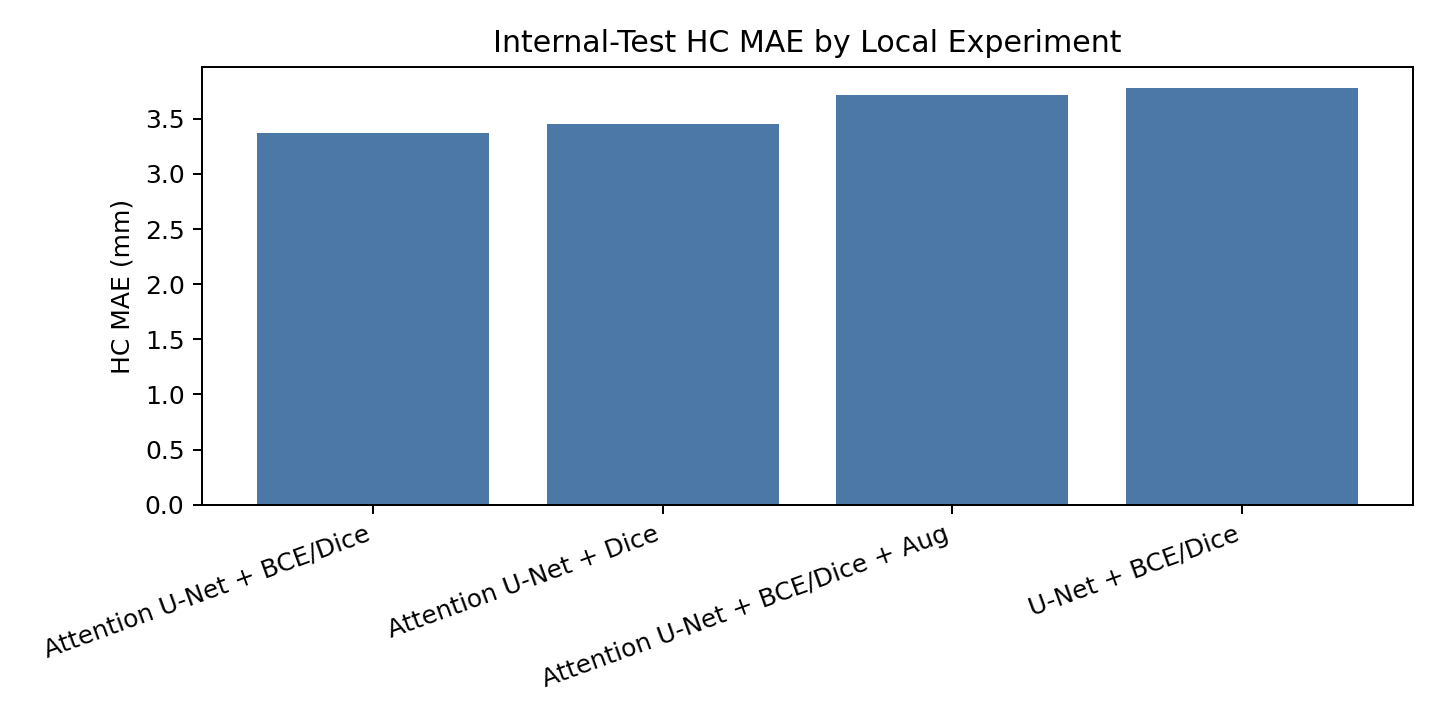
\includegraphics[width=0.72\linewidth]{figures/main_test_hc_mae.png}
\caption{Internal-test HC MAE by experiment. Lower is better.}
\end{figure}

\subsubsection{Post-Processing Ablation}\label{post-processing-ablation}

Because the project goal is HC measurement, I also evaluated measurement
variants after segmentation. Table 2 compares direct contour measurement
against ellipse-based measurement for the best model.

\begin{table}[H]
\centering
\small
\begin{tabular}{lrr}
\hline
Post-processing variant & HC MAE (mm) & HC RMSE (mm) \\
\hline
Cleaned ellipse & \textbf{3.37} & \textbf{4.68} \\
Raw ellipse & 3.37 & 4.68 \\
Cleaned contour & 14.04 & 16.18 \\
Raw contour & 16.73 & 21.27 \\
\hline
\end{tabular}
\caption{Internal-test HC measurement error by post-processing variant.}
\end{table}

Direct contour-length measurement strongly overestimated HC. This
happened because binary mask contours are jagged and can include small
noisy regions. Ellipse fitting regularized the predicted boundary into
the clinically relevant head-shape assumption and reduced HC MAE from
16.73 mm for raw contour measurement to 3.37 mm for cleaned ellipse
measurement. In this run, raw-largest-contour ellipse and cleaned
ellipse matched because ellipse fitting already used the largest
external contour. The important conclusion is that ellipse fitting, not
raw contour length, should be used for the final HC measurement.

Figure 2 shows the same post-processing ablation graphically. The large
gap between contour-based measurement and ellipse-based measurement
shows that the deterministic geometry stage is not cosmetic; it is
essential for turning a segmentation mask into a reliable clinical-style
HC estimate.

\begin{figure}[H]
\centering
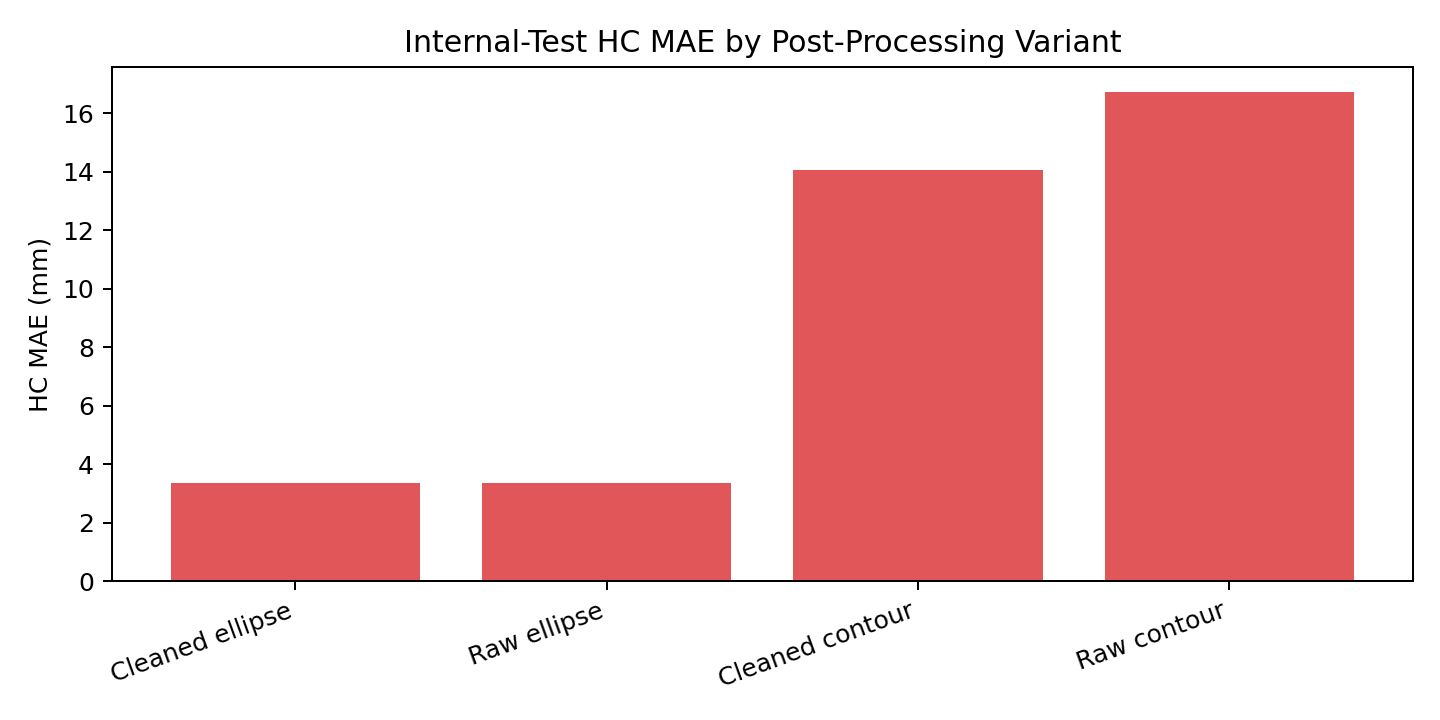
\includegraphics[width=0.72\linewidth]{figures/postprocess_test_hc_mae.png}
\caption{Internal-test HC MAE by post-processing variant. Lower is better.}
\end{figure}

\subsection{4. Conclusions}\label{conclusions}

This project implemented a complete PyTorch pipeline for automatic fetal
head circumference measurement from HC18 ultrasound images. The best
local model was Attention U-Net trained with BCE+Dice loss, followed by
largest-component cleanup and ellipse-based geometric measurement. This
model achieved internal-test Dice 0.9669 and HC MAE 3.37 mm under a
reduced-resource local setup.

The experiments show that segmentation architecture and post-processing
both matter. Attention U-Net improved over the U-Net baseline, while
Dice-only loss and the tested simple augmentation did not improve HC
error. The post-processing ablation was especially important: direct
contour length produced large overestimates, while ellipse fitting
produced much lower measurement error.

The main limitation is compute scale. The v1 results used reduced image
resolution, smaller model width, and 10 training epochs on a MacBook MPS
backend. Future work should rerun the same pipeline on CHPC with larger
images, wider models, and longer training. Other useful extensions
include tuning augmentation strength, inspecting high-error cases,
evaluating official challenge-style test submissions, and building a
lightweight demo for presentation.

\subsection{References}\label{references}

\begin{enumerate}
\def\labelenumi{\arabic{enumi}.}
\tightlist
\item
  Thomas L. A. van den Heuvel, Dagmar de Bruijn, Chris L. de Korte, and
  Bram van Ginneken. ``Automated measurement of fetal head circumference
  using 2D ultrasound images.'' \emph{PLOS ONE}, 13(8), e0200412, 2018.
\item
  HC18 Grand Challenge. https://hc18.grand-challenge.org/
\item
  Thomas L. A. van den Heuvel, Dagmar de Bruijn, Chris L. de Korte, and
  Bram van Ginneken. ``Automated measurement of fetal head circumference
  using 2D ultrasound images'' {[}Data set{]}. Zenodo. DOI:
  10.5281/zenodo.1327317. https://doi.org/10.5281/zenodo.1327317
\item
  Olaf Ronneberger, Philipp Fischer, and Thomas Brox. ``U-Net:
  Convolutional Networks for Biomedical Image Segmentation.'' MICCAI,
  2015. arXiv:1505.04597.
\item
  Ozan Oktay et al.~``Attention U-Net: Learning Where to Look for the
  Pancreas.'' arXiv:1804.03999, 2018.
\item
  Adam Paszke et al.~``PyTorch: An Imperative Style, High-Performance
  Deep Learning Library.'' NeurIPS, 2019. arXiv:1912.01703.
\end{enumerate}

No external public model code was copied for this project; the U-Net and
Attention U-Net implementations are project-local PyTorch modules based
on the published architectures.

\end{document}
